\section{Base de datos de señales de habla y ruido}
\label{sec:audio_db}

Para poder entrenar, comparar y evaluar los algoritmos de supresión de ruido es necesario contar con una base de datos de señales de habla y otra de ruidos. Contando con ambas bases es posible generar una base de datos de señales de habla ruidosa que se utilizarán como la señal de entrada a los filtros.

A la salida de los filtros se obtendrá una señal de habla procesada o filtrada la cual se la comparará con la señal de habla sin ruido utilizando las métricas descritas en la sección \ref{sec:metrics}

\subsection{Señales de habla}

Las señales de habla sin ruido fueron tomadas de \cite{a_scalable_noisy_speech_dataset_and_online_subjective_test_framework} las cuales a su vez se basan en la base de datos creada en la Universidad de Edimburgo \cite{the_voice_bank_corpus}. 

La base de datos consiste en más de 20000 oraciones leídas en voz alta por 56 oradores, 28 masculinos y 28 femeninos. Las oraciones tienen una duración media de aproximadamente 2.6 segundos y se encuentran muestreadas a 16 KHz. Las oraciones consisten en su mayoría de extractos del diario Scottish Herald

\subsection{Señales de ruido}

Como vimos en \ref{sec:objetivos}, el presente trabajó se limitó a estudiar el desempeño de los filtros en señales de habla corrompidas con cuatro tipos de  ruidos presentes usualmente en videoconferencias:

\begin{itemize}
	\item Tipeo: Ruido generado al escribir en un teclado.
	\item Personas hablando de fondo: Presente usualmente cuando un participante se encuentra en un ambiente público como puede ser un café.
	\item Ruido de tráfico y a calle: Ruido presente cuando un participante se encuentra en la vía pública.
	\item Ruidos generados por mascotas: Presentes usualmente en videoconferencias domésticas. En particular se utilizaron ladridos de perro o maullidos de un gato.
\end{itemize}

Las señales de ruido fueron tomadas de 3 bases de datos distintas:

\begin{enumerate}
	\item La base generada por Microsoft en \cite{a_scalable_noisy_speech_dataset_and_online_subjective_test_framework}
	\item Freesound: https://freesound.org/
	\item Google AudioSet: https://research.google.com/audioset/
\end{enumerate}

De (1) se obtuvieron señales de ruido correspondientes a la clase \emph{ruido de fondo} y \emph{tipeo}.

De (2) se obtuvieron más señales correspondientes al ruido \emph{tipeo}

De (3) se obtuvieron las clases \emph{tráfico} y \emph{mascotas}

Al igual que las señales de habla, todas las señales de ruido fueron muestreadas a 16 kHz

\subsection{Generación de señales de habla ruidosas}
\label{sec:noisy_signals_generation}

Como dijimos al comienzo de la presente sección, a partir de la base de señales de habla y de la base de señales de ruidos es posible generar la base de señales de habla ruidosa. 

Los algoritmos se desempeñarán de manera diferente dependiendo del nivel de ruido ($SNR$) que tenga cada una de las señales procesadas. El presente trabajo se limitó a trabajar con el siguiente conjunto de niveles $SNR$

\begin{equation*}
	\{ \SI{-5}{dB}, \; \SI{0}{dB}, \; \SI{5}{dB}, \; \SI{10}{dB}, \; \SI{15}{dB}, \; \SI{20}{dB}, \; \infty \, \si{dB} \}
\end{equation*}

El caso $SNR = \infty \, \si{dB}$ describe el caso de señales de habla sin ruido. Este caso se lo incluye por el hecho de que se busca que los algoritmos no distorsionen señales que no contienen ruido.

\subsubsection{Mezcla de señales a distintos SNRs}

El primer paso para mezclar la señal de habla con la señal de ruido es normalizar ambas señales de tal manera que tengan el mismo valor RMS. A este proceso se le llama normalización RMS y permite mezclar señales que parten del mismo nivel RMS.

Dada una señal de habla $s[k]$ y una señal de ruido $n[k]$, supongamos que se quiere hallar $c_1$ tal que la señal $c_1 \; s[k]$ tenga cierto valor $RMS$ igual a $b$, es decir 

\begin{equation*}
	RMS\{c_1 \; s[k]\} = b
\end{equation*}

El valor RMS de la señal escalada viene dado por:

\begin{equation*}
	b = \sqrt{\frac{1}{K} \sum_{\forall k} (c_1 \; s[k])^2}
\end{equation*}

entonces

\begin{equation*}
	c_1 = \sqrt{\frac{K \; b^2}{\sum_{\forall k} s[k]^2}} = \frac{b}{RMS\{s[k]\}}
\end{equation*}

El valor RMS escogido fue de $\SI{-25}{dB}$, entonces el factor $c$ se obtiene como:

\begin{equation*}
	c_1 = \frac{10^{\frac{-25}{20}}}{RMS\{s[k]\}}
\end{equation*}

Finalmente obtenemos

\begin{equation*}
	s'[k] = \frac{10^{\frac{-25}{20}}}{RMS\{s[k]\}} \; s[k] \qquad \text{y} \qquad n'[k] = \frac{10^{\frac{-25}{20}}}{RMS\{s[k]\}} \; n[k]
\end{equation*}

El segundo paso es mezclar ambas señales a un determinado valor de $SNR$. Para ello debemos calcular el factor de escalado $c_2$, a aplicar en la señal de ruido, tal que

\begin{equation*}
	SNR = \frac{RMS\{s'[k]\}}{RMS\{c_2 \; n'[k]\}}
\end{equation*}

entonces

\begin{equation*}
	c_2 = \frac{RMS\{s'[k]\}}{SNR \quad RMS\{n'[k]\}}
\end{equation*}

y dado que usualmente el valor $SNR$ es expresado en $\si{dB}$ tenemos que:

\begin{equation*}
	c_2 = \frac{RMS\{s'[k]\}}{10^{\frac{SNR}{20}} \quad RMS\{n'[k]\}}
\end{equation*}

Luego se obtiene la señal de habla ruidosa calculando:

\begin{equation*}
	y'[k] = s'[k] + c_2 \; n'[k]
\end{equation*}

Por último es necesario contar con señales de habla ruidosas con distintas intensidades, por lo tanto se realizó una nueva normalización RMS con un valor objetivo aleatorio de entre $\SI{-15}{dB}$ y $\SI{-35}{dB}$. Dado $l$ el valor RMS aleatorio en decibeles, el factor de escalado se calcula como:

\begin{equation*}
	c_3 = \frac{10^{\frac{l}{20}}}{RMS\{y[k]\}}
\end{equation*}

Finalmente la señal de habla ruidosa viene dada por:

\begin{equation*}
	y[k] = c_3 \left( s'[k] + c_2 \; n'[k] \right)
\end{equation*}

\subsubsection{Niveles base de PESQ y STOI}

Cada señal de habla ruidosa tendrá cierto nivel base para las medidas PESQ y STOI. El objetivo de los algoritmos de supresión de ruido es mejorar el nivel base.

Dependiendo de las características de cada señal ruidosa, el nivel base será diferente.

Las figuras \ref{fig:ch5_pesq_histogram} y \ref{fig:ch5_stoi_histogram} muestran un histograma de los niveles base para los distintos valores de SNR utilizados

\begin{figure}[H]
	\centering
	\centerline{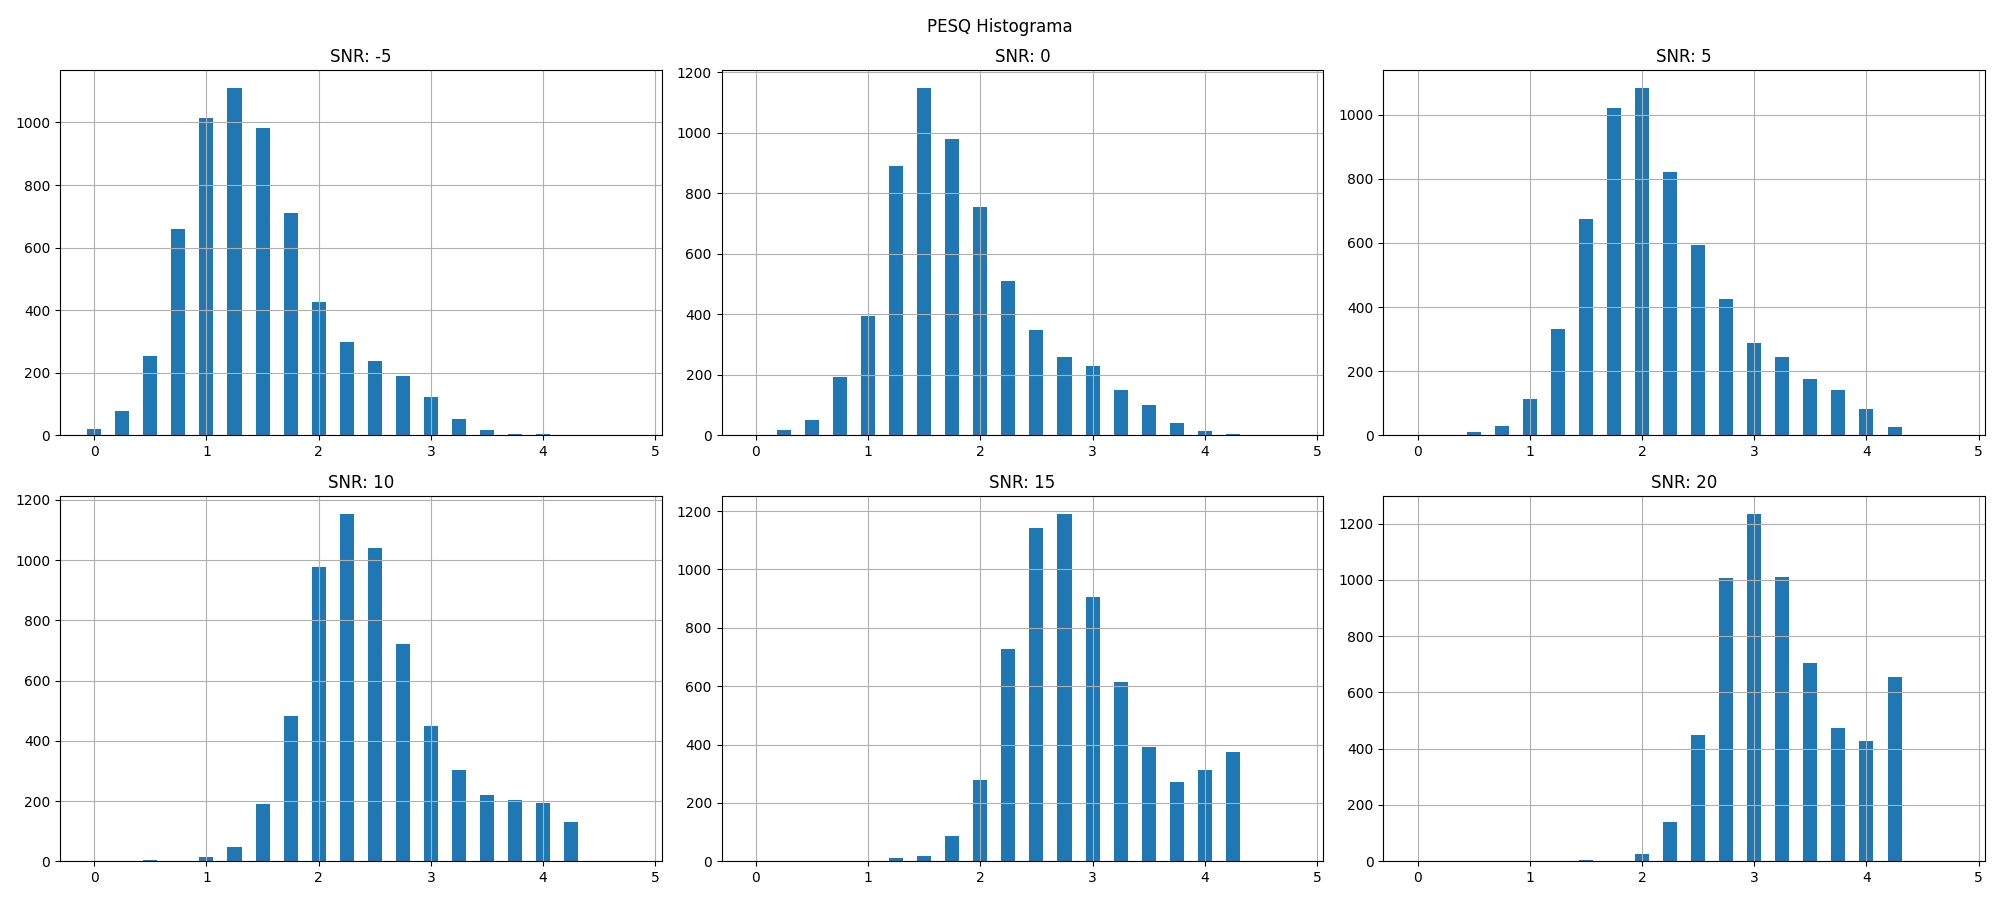
\includegraphics[scale=0.35]{images/ch5/pesq_aggregated.png}}
	\caption{Histograma PESQ}
	\label{fig:ch5_pesq_histogram}
\end{figure}

\begin{figure}[H]
	\centering
	\centerline{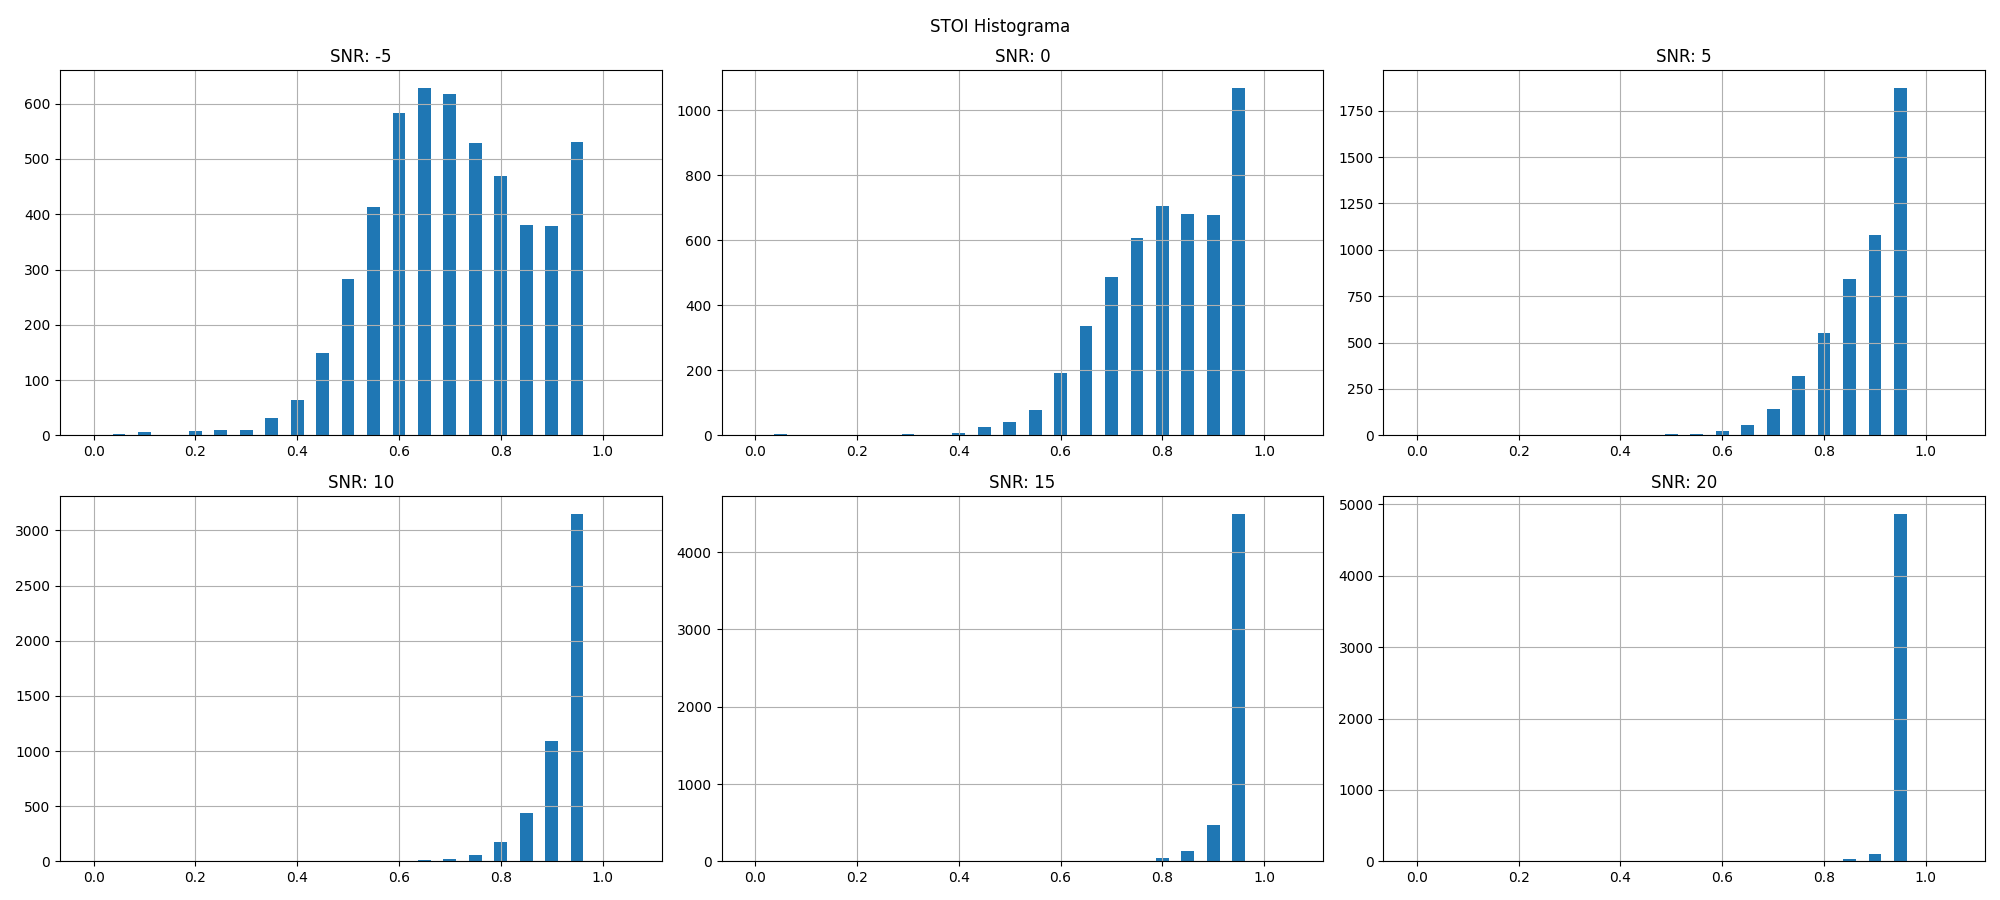
\includegraphics[scale=0.35]{images/ch5/stoi_aggregated.png}}
	\caption{Histograma STOI}
	\label{fig:ch5_stoi_histogram}
\end{figure}

A medida que la SNR aumenta, los valores medio de PESQ y STOI se corren hacia la derecha, es decir se acercan al valor máximo el cual para PESQ es de 4.5 y para STOI es de 1. Ambos límites son alcanzados cuando la SNR es infinita, es decir cuando no hay presencia de ruido en la señal de habla.

\subsection{Ruido correlacionado}

Como vimos en la sección \ref{sec:adaptive_filter_architecture}, el filtro adaptativo depende de dos señales de entrada, la señal de habla ruidosa $d(n)$ y la señal de ruido correlacionado $u(n)$. 

En la sección anterior vimos cómo se construyeron las señales de habla ruidosa mezclando señales de habla con señales de ruido, las cuales fueron obtenidas de bases de datos comúnmente utilizadas en experimentos relacionados con el presente trabajo. Sin embargo, para el caso de ruido correlacionado, no fue posible encontrar una base de datos obtenida a partir de grabaciones reales y se optó para fabricar la base a partir de la base de señales de ruido.

Para fabricar el ruido correlacionado lo que se hizo fue partir la señal de ruido en bloques de largo aleatorio en el conjunto \{16384, 32768, 65536\}. Luego a cada bloque se le aplicó un filtro $A$, nuevamente, de largo aleatorio en el rango [8, 12] cuyos coeficientes también son aleatorios en el rango [0, 1].

En una configuración como la que vimos en la figura \ref{fig:ch3_af-se-setup}, en algunas ocasiones es posible que ocurra el fenómeno de diafonía donde parte de la señal de habla $s(n)$ se mezcla con el ruido de referencia $n_2(n)$. Para simular condiciones similares a las encontradas en la práctica, además de realizar la transformación aleatoria descrita en el párrafo anterior, a la señal obtenida se le sumó un porcentaje $a$, de la señal de habla $s(n)$ aleatorio en el rango [0, 5].

Resumiendo, la señal de ruido de referencia fue obtenida como:

\begin{equation*}
	n_2(n) = A(n) \circledast n_1(n) + a(n) \cdot s(n)
\end{equation*}

\noindent donde $A(n)$ son los filtros aleatorios y $a(n)$ son los coeficientes aleatorios de diafonía.